\documentclass[a4paper,12pt]{article}

\usepackage{url}
\usepackage{epsfig}
\usepackage{graphics}
\usepackage{fancyhdr}
\usepackage{amsmath}
\usepackage{pdflscape}
\usepackage{longtable}
\usepackage[noend, linesnumbered]{algorithm2e}


\graphicspath{{pictures/}}

\title{Detecting context-dependent word defects in written English by native Swedes with n-grams}
\author{\hspace*{-0.5cm}\begin{tabular}{cccc}
Frej Connolly & Maja Gidlund & Sandra Liljeqvist & Sara Norrby \\
connolly@kth.se & majagi@kth.se & sanlil@kth.se & saranorr@kth.se \\
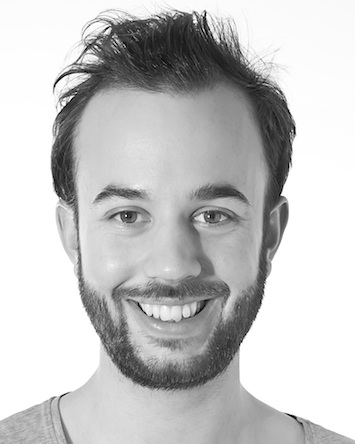
\includegraphics[width=0.13\linewidth]{frej} & 
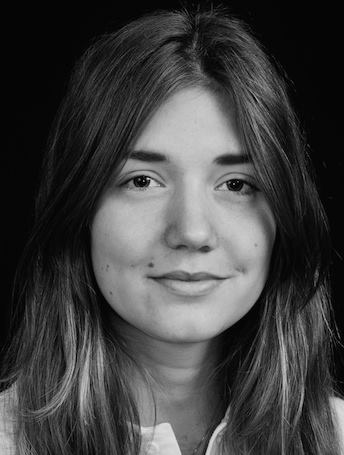
\includegraphics[width=0.13\linewidth]{maja} & 
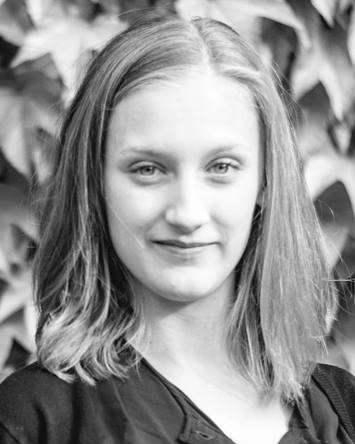
\includegraphics[width=0.13\linewidth]{sandra} & 
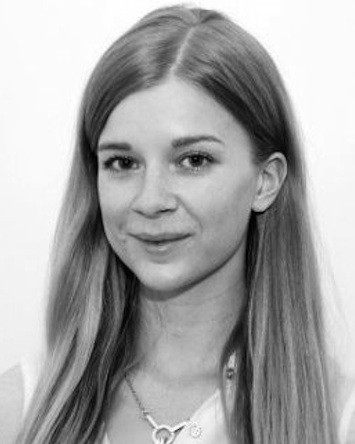
\includegraphics[width=0.13\linewidth]{sara}
\end{tabular}}
\date{2014-10-20}

\pagestyle{fancy}
\setlength{\headheight}{15pt}
\fancyhf{}
\lhead{DD2380 ai14} % DO NOT REMOVE!!!!
\rhead{F. Connolly, M. Gidlund, S. Liljeqvist, S. Norrby}

\begin{document}

\maketitle
\thispagestyle{fancy}

\begin{abstract}
There is a growing need to be able to write accurate English as the market is becoming more global. For people that have English as a foreign language this can involve issues that a normal spell checker will not detect, for example words that are correctly spelled but is out of context. In this paper we use n-gram modeling to determine whether bigrams are sufficient in order to detect this type of errors made by native Swedes. The result of our work shows that bigrams are sufficient if the error occurs between two adjacent words. However, if the error occurs in two different parts of a sentence it is not. Our work also shows the importance of using a large corpus in order to be able to use n-grams with good results.
\end{abstract}



\clearpage

%%%%%%%%%%%%%%%%%%%%%%%%%%%%%%%%%%%%%%%%%%%%%%%%%%%%%%%%%%%%%
%%%%%%%%%%%%%%%%%%%%%%%%%%%%%%%%%%%%%%%%%%%%%%%%%%%%%%%%%%%%%
\section{Introduction}
\label{sec:introduction}
The need to be able to write accurate English is growing as the market is becoming more global. For non-native speakers it is easy to write words that do not make sense in a certain context. One example of a common cause of this is, so called, false friends. This is e.g. if a Swede would like to ask a friend if he has a tuxedo and the person says \emph{Do you have a smoking?} believing that the word smoking (Swedish word for tuxedo) has the same meaning in English. The native English speaker could interpret that what the Swede really is saying is \emph{Do you have a cigarette?}.  

Another type of mistake could be that the writer misspelled a word in a way that it transformed into another existing word, different from what the writer intended. This type of errors is called real-word errors. The problem is that a traditional spell checker, that only checks for words not occurring in a dictionary, would not recognize this word as a misspelling since the word itself is correct but placed in the wrong context. A third type of common problems are errors caused by using incorrect grammar.  

The aim for this study is to construct an algorithm that is not only looking for misspelled words, but also detects the previously mentioned problems. We anticipate that a tool that can discover these kinds of mistakes could be of a great help for people who do not have English as their first language. The tool could be used for detecting context-dependent word defects in terms of grammatical spelling errors, real-word errors and false friends.

One way to implement this type of word detection is by using n-grams. This is done by combining the words that is next to each other in a sentence. Common lengths are unigram $(n=1)$, bigrams $(n=2)$ and trigrams $(n=3)$. A list of previously computed n-grams are often used when trying to predict the next word when writing a sentence \cite{gallagher2004natural}. This is covered in more detail later on in the report section \ref{sec:ngram}

\subsection{Objective}
\label{sec:objective}
The aim for this project is to investigate if an algorithm, using bigrams, can find words that are out of context due to grammatical spelling errors, real-word errors and false friends. We will analyze if this algorithm can identify this kind of mistakes in different sentences, both correct and incorrect ones. The application area will be for people with Swedish as a first language and English as a foreign language and focus on the type of errors that Swedes often do. 

\subsection{Hypothesis}
Our hypothesis is that it is enough to use bigrams to detect words that are out of context in a given text. However, the results will be dependent on the quality of the corpus (covered in section \ref{sec:ngram}) and we believe that a large and well chosen corpus is vital for the result of this study.

As the investigation focuses on the context, the use of unigrams would not be relevant, since it is only based on the current word. On the other hand, finding larger n-grams with many words in a row is rare and could create false positives. Therefore we decided to use bigrams. We chose to not use trigrams or larger n-grams since the amount of data required for trigrams is much larger than the amount for bigrams and the result is dependent on the quality of the corpus and the amount of n-grams that we can generate. However, bigrams may not be enough to capture the context of the sentence. 

\subsection{Contribution}
\label{sec:contribution}
Previous research has been done in this field and with different focus areas. These have, for example, been different techniques or a specific language. However, no paper has been found that focuses on the Swedish languages and the difficulties that people with Swedish as their first language have with English. It is of interest to investigate this since we cannot say that the results of research made for other languages is definitely applicable to Swedish as well. The focus of our study also includes aspects that we have not seen in earlier work, since we focus on false friends as well as real-word errors and grammatical errors. Earlier studies have mainly used trigrams in their work and we have chosen to use bigrams to see if this could be sufficient. 

\subsection{Outline}
\label{sec:outline}
In section \ref{sec:languagemodeling} we describe the n-gram model and give a more detailed explanation of what false friends and real-word errors are.  In section \ref{sec:relatedwork} we discuss the previous work in the same field. We go into some detail of the methods used by research similar to ours and highlight the similarities and differences. In section \ref{sec:method} we present our method, what resources we used and how success should be measured in the experiments. In section \ref{sec:experimentalresults} we discuss the experimental setup and present the results of our experiments. The results are discussed and possible improvements are suggested. In section \ref{sec:summary} we summarize our work and draw conclusions from the results. 

\section{Language Modeling}
\label{sec:languagemodeling}
To be able to develop the algorithm, some language modeling techniques were used, which are described in the following section.

\subsection{N-gram modeling}
\label{sec:ngram}
In general a statistical language modeling is based on n-gram modeling which tries to predict the next word based on the $n-1$ previous words in the sentence\cite{gallagher2004natural}.  When choosing one previous word to compute the probability that a given word is the next word, it is called bigrams. If we for example have the sentence \emph{I painted the house in the color} and uses bigram to guess the next word in the sentence we would compute $P(\emph{predicted-word}| \emph{color})$. Although it makes more sense to assume, by using the whole sentence, that it would be easier for a human to guess the next word. This because the guess could then also be based on the context of the sentence. However, the bigram does not take as much computer power unlike if one wants to compute the whole sentence. It also takes less time to compute a bigram in comparison to compute a whole sentence\cite{gallagher2004natural}.

The information that is needed to compute an n-gram is how often a word occurs in general and how often a word occurs with others specific words. The n-gram model is using the Markov assumption, which is the assumption that the future behavior of a dynamical system only depends on its recent history \cite{mooneynatural}. In this case the history of the $n-1$ previous words. 

The n-gram model is often used together with one or several corpora. This is a large collection of text, written by humans, for different purposes that can be used for analyzing natural language. A great volume of text like this is necessary to make a probabilistic model, like n-grams, effective, since this approach requires that the system is learning from a big amount of data\cite{RussellNorvigAIBook}.

\subsection{False friends and real-word errors}
False friends contribute to the difficulties of using certain words in the right context in a foreign language. The paper \emph{Automatic Identification of Cognates and False Friends in French and English} by Diana Inkpen and Oana Frunza brings up false friends and cognates. In most languages there are words that are similar, in spelling, to words in other languages. Sometimes this can be helpful, cognates are pairs of words in two different languages that have similar spelling and also the same meaning \cite{inkpen2005automatic}. One example is the Swedish word for nature (Swe. \emph{natur}). They have the same meaning and almost the exact spelling. False friends are words that have similar spelling but completely different meaning, one example is the Swedish word \emph{delikat} which means delicious, but looks more like the word delicate.

Real-word errors are errors made while writing, which results in another word. This results in words that are correct but out of context in the sentence. A few studies have been made that explore the frequency of the occurrences of this type of error, and it ranges from 25 % to 40 % of the errors that were examined. An example of this type of error is typing the word \emph{form} instead of \emph{from}.\cite{Kukich}

\section{Related work}
\label{sec:relatedwork}
A field related to ours is word prediction, it has been covered in several studies with different approaches. One of them is described in the paper \emph{User Interaction with Word Prediction: The Effects of Prediction Quality} by Trnka McCaw, Yarrington and McCoy in 2009. Their hypothesis is that word prediction can be used to increase the communication rate for people that need alternative communication methods and that the accuracy of the predictions is crucial for this to be true. Their method was to compare two algorithms, of different complexity, with normal typing without any predictions. The basic algorithm was to suggest words that had been used previously. The more advanced algorithm was using trigram language modeling where the prediction was based on the statistics generated from a corpus. The conclusion was that word prediction can be used to improve the typing speed and that the advanced prediction technique was the one that reduced the number of keystrokes the most \cite{trnka2009user}. The result from this study made it clear to us that n-grams are effective for word prediction and that it probably also could be used in our work.

Several research papers have discussed how to capture the context of a sentence without having to analyze the whole sentence. In the article \emph{A Swedish Grammar for Word Prediction} (2003), written by Ebba Gustavii and Eva Pettersson, grammar rules was implemented by using the FASTY language modeling to predict the next word with the use of the n-gram modeling \cite{gustavii2003a}. FASTY is an intelligent system, which uses methods of Natural Language Processing, to increase keystroke saving rate (KSR) \cite{fasty}.  The article's aim was to improve the cover contexts where statistical models gives irrelevant suggestions of the next word and therefore achieve a better value of KSR. However the result showed a small improvement of the KSR after implemented the grammar module FASTY to the system comparing with the use of bigram and part-of-speech tag trigram. This also confirms our choice of using n-grams as a method in this study, although others knowledge-based approaches have been developed in the area of natural language modeling. \cite{gustavii2003a}

Even though this study does not focus on spelling correction, there has been other studies using similar techniques to achieve this. One example is the paper \emph{Context Based Spelling Correction} by Mays et al. from 1991. They are using a statistical language modeling approach to detect and correct words that are out of context due to misspelling.  Probability estimation, for the trigrams that they use, was done with a large corpus. In their experiment they generated sentences containing one real-word error from a set of correct sentences, and then compared the faulty sentence probability to the correct sentence. In some cases, where the generated bad sentence was plausible, they were not able to find or correct the misspelled word. However they were able to detect 76 \% of simple spelling errors that resulted in real-word errors. The method they use is similar in the sense that they also use n-grams but the n-grams are constructed with pragmatic, syntactic and semantic knowledge with conditional probabilities. The way they test their algorithm is suitable for our work as well.\cite{Mays1991}

Also studies about word correction have been made. The paper \emph{Techniques for automatically correcting words in text} by Karen Kukich (1992) brings up three different types of error detection and correction., non-word error detection, isolated-word error correction and context dependent word-correction. The latter being the most interesting to us. As an example of how this kind of errors occur mentioned by Kukich, is the situation when a word is misspelled in such a way that it becomes another one, grammatical or syntactic mistakes in shape of use of the wrong inflected form or the wrong function word etc. Kukich discusses previous work and different approaches for the context dependent word-correction, she mentions an alternative to context dependent word-correction approaches, which is an statistical language modeling approach using n-grams. The difference between the approaches is that statistical language modeling is based on probabilities and context dependent word-correction approaches are based on philosophical observations and grammatical or syntactical rules. \cite{Kukich1992Tecniques}.

In the paper\emph{Correcting real-word spelling errors by restoring lexical cohesion}, Hirst and Budanitsky propose a new algorithm for detecting real-word errors. Their algorithm is bidirectional and does therefore recognize the potential cohesion between the beginning and end of a sentence.  They make the assumptions that the intended word is semantically related to the words nearby and that it is unlikely that the word is completely unrelated to all words that are nearby, and that the error is unlikely to be semantically related to the surrounding text. They do not however use n-grams and their algorithm is therefore somewhat unrelated to ours. \cite{hirst}

Previous work on predicting the next word when typing have been using different methods measuring success. Some of the common ones includes hit rate and keystroke saving (KSS) \cite{ghayoomi2005word}. In the context of predicting the next word, hit rate is the percentage of correct words that appear before writing any letters of the next word. Keystroke saving is the number of keystrokes saved by using the word prediction program.  Higher value means better performance on both. Many other orthographic similarity methods have been evaluated before \cite{frunza2006automatic}. The goal of most of them is to quantify the human perception of similarity, which is quite subjective. In our work we decided to use hit rate since it is a good method to evaluate how successful an algorithm is in this field of study, as it has been used in work similar to ours. 

\section{Method}
\label{sec:method}
The project is divided into two parts: implementation and analyzing.

\subsection{Implementation}
\label{ref:implementation}
The implementation is based on the previously mentioned n-gram model. Based on the hypothesis, bigrams was used to be able to find plausible incorrect words. The text processing library Natural Language Toolkit (NLTK) in Python is conveniently used to save time for already solved problems. It is a platform for language modeling and it provides many corpora, lexical resources and provides common NLP functions\cite{loper2002nltk}. 

To create a good library of bigrams  two corpora and a list of most frequently bigrams were used.  The Brown corpus contains 1,15 million words which is gathered from works published in the United States in 1964\cite{francis64brown}. The web text corpus used contains 200 000 words text with less formal language with content extracted from discussions, movie scripts, wine reviews etc. \cite{nltkWebtext}. The data set was further improved by using the 286 000 most frequently used bigrams from websites collected by Google in \emph{Google Web Trillion Word Corpus} \cite{google}.  This resulted in a total set of bigrams of 627 353. 

\subsection{Analyzing}
\label{ref:analyzing}
A bigram was considered to be proper English if it was included in the constructed bigram library, and incorrect if it was not. A more advanced statistical method could not be used since it would require a larger corpus. 

For measuring the results we calculated the quota between the correctly detected defects and all defects together with incorrectly detected defects. This equation is called \emph{hit rate} \cite{ghayoomi2005word}.

$$z = \frac{\sum correct}{\sum correct + \sum not\_detected + \sum incorrect}$$
\begin{description}
  \item[correct] \hfill \\
  		correctly detected defects
  \item[not\_detected] \hfill \\
  		defects not detected
  \item[incorrect] \hfill \\
   		incorrect defects detected
\end{description}

If $z$ equals one, the algorithm correctly found all defects with no incorrect matches and if z is zero, it did not found any of the defects.

For the experiment we used both incorrect sentences and the corresponding correct version of each sentence. The sentences were constructed as simple sentences with one incorrect word in each one. The incorrect words were false friends, real-word errors or grammatical errors. In the correct sentences, these incorrect words, were replaced with the word that made sense in the sentence. 

For the hit rate calculation of the incorrect sentences, the true positives are the correctly detected defects, the negative positives are the defects that are not detected and false positives are the incorrect defects detected words in Algorithm 1. In a similar way, the true positives, for the correct sentences, are the total number of bigrams except the found defects, zero false negatives and false positives the number of found defects Algorithm 2.
 
\begin{figure}[h]
\begin{algorithm}[H]
    \DontPrintSemicolon
    \SetKwFunction{KwFn}{hitrateincorrect}
    \SetAlgoLined
    \renewcommand\bottomfraction{0.85}
    \KwData{sentence = text to measure containing exactly one wrong word,
				  wrong\_word = word in sentence that does not make sense,
            	  library = set of bigrams constructed from corpus}
    \KwResult{Hit rate for sentence $n$}
    \SetKwFunction{hitrateincorrect}{hitrate\_incorrect\_sentence}
    \SetKwProg{myhitrateincorrect}{function}{}{}
    \myhitrateincorrect{\hitrateincorrect{sentence, wrong\_word, library}}{
		$bigrams \leftarrow$ construct\_bigrams(sentence)\;
		$correct\_defects \leftarrow$ bigrams containing wrong\_word\;		
		$found\_defects \leftarrow$ bigrams not in library\;
		$incorrect \leftarrow$ count(found\_defects not in correct\_defects)\;
		\If{any correct\_defects in found\_defects}{
			$correct \leftarrow 1$\;
			$not\_detected \leftarrow 0$\;
        }
        \Else{
			$correct \leftarrow 0$\;
			$not\_detected \leftarrow 1$\;
        }				
		\Return{correct / (correct + not\_detected + incorrect)}
    }
    \caption{Calculate hitrate for the sentences containing exactly one wrong word.}
\end{algorithm}
\end{figure}

\begin{figure}[h]
\begin{algorithm}[H]
    \DontPrintSemicolon
    \SetKwFunction{KwFn}{hitratecorrect}
    \SetAlgoLined
    \renewcommand\bottomfraction{0.85}
    \KwData{sentence = text to measure containing no errors,
            	  library = set of bigrams constructed from corpus}
    \KwResult{Hit rate for sentence $n$}
    \SetKwFunction{hitratecorrect}{hitrate\_correct\_sentence}
    \SetKwProg{myhitratecorrect}{function}{}{}
    \myhitratecorrect{\hitratecorrect{sentence, library}}{
		$bigrams \leftarrow$ construct\_bigrams(sentence)\;
		$found\_defects \leftarrow$ bigrams not in library\;
		$incorrect \leftarrow$ count(found\_defects)\;
		$correct \leftarrow $ count(bigrams) - incorrect\;
		$not\_detected \leftarrow 0$\;
		\Return{correct / (correct + not\_detected + incorrect)}
    }
    \caption{Calculate hitrate for the sentences containing exactly one wrong word.}
\end{algorithm}
\end{figure}

%%%%%%%%%%%%%%%%%%%%%%%%%%%%%%%%%%%%%%%%%%%%%%%%%%%%%%%%%%%%%
%%%%%%%%%%%%%%%%%%%%%%%%%%%%%%%%%%%%%%%%%%%%%%%%%%%%%%%%%%%%%
\section{Experimental results}
\label{sec:experimentalresults}

\subsection{Experimental setup}
In the experiment we did test runs for both the incorrect and the correct sentences. This was done to ensure that we got a more accurate estimation of how successful our application was and also to be able to see differences between the two types. We used 51 sentences of each type and in the construction of the sentences the focus was on typical errors that Swedes often do. These can be seen in appendix \ref{appendix:A}.

\subsection{Experiment}
The results of the experiment is shown in the table \ref{table:results} below. Briefly it indicates that the algorithm gives a higher hit rate of the correct sentences than the incorrect sentences. A more detail description of the results for the two sets of test data will be presented, as well as an analysis of the both results. A complete list of the results can be found in appendix \ref{appendix:A}.

\begin{table}[h]
\begin{center}
\begin{tabular}{lllll}
\hline
Type & Correct & Not detected & Incorrect & Hit rate \\
\hline
Incorrect sentences & 34 & 17 & 14 & 0,523  \\
Correct sentences & 213 & 0 & 45 & 0,825  \\
\hline
\end{tabular}
\caption[Table caption text]{The hit rate for the correct and incorrect sentences}
\label{table:results}
\end{center}
\end{table}

The result for the correct sentences was 0.825 in hit rate. This result shows that there are some flaws in our algorithm since the hit rate should be 1. Out of the 51 correct sentences our algorithm found false positives in 33 of them.

One of the sentences with 1 in hit rate was \emph{I work as a photographer}, the algorithm found no defects as expected. The sentence \emph{Do you have a tuxedo} with hit rate 0.75, had a defect (a, tuxedo). In the sentence \emph{He checks passports for the airport} with hit rate 0.4, our algorithm found three defects: (he, checks), (checks, passports), (passports, at). These results are exclusively dependent upon the corpus that we used to check whether a combination of words is valid or not. The fact that the algorithm cannot correctly evaluate correct sentences should be kept in mind when reading the result for the incorrect sentences.

The result from the incorrect sentences had a hit rate of 0.523, which implies that approximately half of the found errors were correctly detected. One example of a correctly detected sentence is \emph{These are my barns} (the correct expression would be \emph{These are my children}) where the algorithm found and pointed out (my, barns) as an incorrect bigram. 

An example where the algorithm on the other hand did not work as expected was in \emph{I think I will jump over the tea this morning} where the bigram (tea, this) was found and not (jump, over) which is a literally translated Swedish expression. From this, two conclusions can be made. The first is that \emph{tea this} may not be a common phrase, even though it is not incorrect, and does not exist in our corpus, which makes it a false positive. The second aspect is that the phrase \emph{jump over} is a correct expression that can be used in a different contexts, for example if you would jump over an object. That is why it was not recognize as defect. 

Another type of problem was found in sentences where the context not is clear from two nearby words. For example in \emph{The door was closed with a smell}. Smell is similar to the Swedish word for bang and is therefore the error in this sentence. However, the problem is the combination of the word \emph{door} and that it was closed with a \emph{smell}. (a, smell) on the other hand, is not an incorrect combination of words although it has a completely different meaning.

\section{Summary and Conclusions}
\label{sec:summary}
The fact that most of our correct sentences had one bigram that was marked as defective is a reflection upon the fact that our corpus is not big enough. A larger corpus would make the number of false positives, generated by our algorithm, decrease and would therefore be desirable to, in a proper way, analyze the algorithm.

For this algorithm no statistical methods, like a threshold for probability of a certain bigram, has been used. This has not been possible because of the small corpus, since we have not even been able to identify all correct bigrams as correct as it is now. With a greater corpus, more sophisticated methods could have been used to find errors and maybe even to interpret the probability for an error to be of a certain type, as a false friend, real-word error or a grammatical error. 

We see in the result that when two adjacent words are a part of the context error, our algorithm works perfectly as it identifies the incorrect bigram. In these cases, bigrams are sufficient. When the context error is further apart, when for example the incorrect word is at the end of a sentence and refers to a word in the beginning of the sentence, our algorithm does not work. To make our algorithm better in the sense that it would discover words in these cases, when the concerned words are not adjacent, we would have to use larger n-grams. The next step would be to try trigrams instead of bigrams. However, we have already recognized that our corpus is too small even for bigrams and the need of a large corpus would increase with a bigger n.

Bigrams are sufficient to find words that are out of context if the incorrect word is adjacent to a word producing the context error. In other cases, bigrams are not sufficient. A larger corpus would solve many of the issues that we have detected and it would vastly improve our result.  

\subsection{Future work}
\label{sec:futurework}
For future work we suggest that an algorithm should be created that can handle data including apostrophes. An apostrophe is not used in the same extent in the Swedish language as in the English language, therefore we assume that is it common that an apostrophe is used incorrect when a Swede express themselves in English. 
 
The used corpora was partly based on the Brown corpus, published 1964, which indicates that new, modern expressions and words that are commonly used today may not exist in the corpus \cite{francis64brown}. This corpus also reflects the structure of the society in the past. This means that the detection of a correct phrase is decided upon if the phrase was commonly used before the 60’s. This means that if we have a sentence that reflects our society of today, the sentence may not exist in the Brown corpus. In other words, the detected errors are highly dependent on the selected corpus and therefore we suggest that a further development of the algorithm would be to not only use n-gram modeling, but also to combine this with at least one other method. This is to reduce the problem of the results being affected by common language and instead be able to focus on finding real defects. 

\bibliographystyle{plain}
\bibliography{reflist}

\begin{landscape}
\fontsize{10}{11}\selectfont
\centering
\appendix
\section{Result incorrect sentences}
\label{appendix:A}
\pagestyle{empty}
\begin{longtable}{l l l r l}
Hitrate & Wrong word & Sentence & Count & Defects found \\
\hline
0,000 & smoking & Do you have a smoking & 0 &  \\
1,000 & pied & It has pied & 1 & (has, pied) \\
1,000 & overdrive & Do not overdrive & 1 & (not, overdrive) \\
1,000 & about & Have you changed about & 1 & (changed, about) \\
0,000 & smell & The door was closed with a smell & 0 &  \\
0,000 & shoot & Can you shoot the window & 0 &  \\
1,000 & strike & Do you want to strike your clothes & 1 & (strike, your) \\
1,000 & bear & I like to eat bear & 1 & (eat, bear) \\
0,000 & jump & I think I will jump over the tea this morning & 1 & (tea, this) \\
1,000 & spoiling & We had a problem spoiling the toilet & 2 & (problem, spoiling), (spoiling, the) \\
1,000 & rapefields & It is probably rapefields & 1 & (probably, rapefields) \\
1,000 & funny & I always have a funny time at parties & 1 & (funny, time) \\
1,000 & disabled & Disabled toilet & 1 & (disabled, toilet) \\
0,000 & are & When are you born & 1 & (you, born) \\
0,000 & diary & Sorry to hear about your diary & 0 &  \\
0,000 & kiss & I need to go the the toilet and kiss & 0 &  \\
1,000 & moose & Can you pass me the potato moose & 1 & (potato, moose) \\
1,000 & call & This morning was very call & 1 & (very, call) \\
0,000 & to & She is a friend to me & 0 &  \\
0,500 & swimming & Could I have some water because my friend is swimming & 2 & (water, because), (is, swimming) \\
0,000 & lend & I need to lend a pen from you & 1 & (pen, from) \\
1,000 & were & were are you & 1 & (were, are) \\
1,000 & learns & He learns children & 1 & (learns, children) \\
0,500 & controls & He controls passports at the airport & 3 & (he, controls), (controls, passports), (passports, at) \\
1,000 & semester & We are going on semester together & 2 & (on, semester), (semester, together) \\
1,000 & drunk & I am back drunk & 1 & (back, drunk) \\
0,500 & table & I like sandwich table & 2 & (like, sandwich), (sandwich, table) \\
1,000 & stark & She is very stark & 1 & (very, stark) \\
1,000 & flipper & I want to play flipper & 1 & (play, flipper) \\
1,000 & pockets & Have you read any good pockets lately & 2 & (good, pockets), (pockets, lately) \\
1,000 & vine & Can I have a glass of vine & 1 & (of, vine) \\
1,000 & basket & Do you want to play basket & 1 & (play, basket) \\
1,000 & backslick & I have my hair in a backslick & 1 & (a, backslick) \\
0,000 & receipt & Can I have the receipt for this soup & 1 & (this, soup) \\
0,000 & photograph & I work as a photograph & 0 &  \\
0,000 & fall & I am investigating this fall & 2 & (am, investigating), (investigating, this) \\
0,000 & rent & What is the rent on your bank loan & 0 &  \\
1,000 & vibrant & My phone is vibrant & 1 & (is, vibrant) \\
1,000 & glass & I like to eat glass & 1 & (eat, glass) \\
0,000 & brick & Put the cups on the brick & 1 & (cups, on) \\
1,000 & island & It is cold in island & 1 & (in, island) \\
1,000 & barns & These are my barns & 1 & (my, barns) \\
1,000 & expedition & I am going to the expedition on the fifth floor & 1 & (expedition, on) \\
0,000 & meaning & Can you write a meaning & 0 &  \\
1,000 & dans & May I have the pleasure of this dans & 1 & (this, dans) \\
0,000 & bio & Would you like to go to the bio & 0 &  \\
1,000 & slang & Use the water slang to water the flowers & 2 & (water, slang), (slang, to) \\
0,500 & bra & It is going to be bra weather tomorrow & 3 & (be, bra), (bra, weather), (weather, tomorrow) \\
0,333 & fond & I have started a fond for you college fees & 3 & (fond, for), (you, college), (college, fees) \\
0,000 & disk & I will do the disk & 0 &  \\
1,000 & mark & Dig a hole in this mark & 1 & (this, mark) \\
\hline
0,531 & total hitrate
% \caption{Result incorrect sentences.}  % Fick inte caption att funka
\label{tab:resultincorrect}
\end{longtable}
\end{landscape}

\begin{landscape}
\centering
\fontsize{10}{11}\selectfont
\section{Result correct sentences}
\pagestyle{empty}
\begin{longtable}{l l r l}
Hitrate & Sentence & Count & Defects found (should be none) \\
\hline
0,750 & Do you have a tuxedo & 1 & (a, tuxedo) \\
1,000 & It broke & 0 &  \\
0,333 & Do not overdo it & 2 & (not, overdo), (overdo, it) \\
0,666 & Have you changed outfit & 1 & (changed, outfit) \\
1,000 & The door was closed with a bang & 0 &  \\
1,000 & Can you shut the window & 0 &  \\
0,833 & Do you want to iron your clothes & 1 & (iron, your) \\
0,750 & I like to eat berries & 1 & (eat, berries) \\
0,750 & I think I will skip the tea this morning & 2 & (will, skip), (tea, this) \\
0,666 & We had a problem flushing the toilet & 2 & (problem, flushing), (flushing, the) \\
0,500 & It is probably rape fields & 2 & (probably, rape), (rape, fields) \\
1,000 & I always have a fun time at parties & 0 &  \\
0,750 & Toilet is out of order & 1 & (toilet, is) \\
0,333 & When were you born & 2 & (when, were), (you, born) \\
0,800 & Sorry to hear about your diarrhea & 1 & (your, diarrhea) \\
0,900 & I need to go the the toilet and have a pee & 1 & (a, pee) \\
0,833 & Can you pass me the mashed potatoes & 1 & (the, mashed) \\
1,000 & This morning was very cold & 0 &  \\
1,000 & She is a friend of mine & 0 &  \\
0,777 & Could I have some water because my friend is fainting & 2 & (water, because), (is, fainting) \\
0,857 & I need to borrow a pen from you & 1 & (pen, from) \\
1,000 & where are you & 0 &  \\
0,500 & He teaches children & 1 & (teaches, children) \\
0,400 & He checks passports at the airport & 3 & (he, checks), (checks, passports), (passports, at) \\
0,800 & We are going on holiday together & 1 & (holiday, together) \\
0,666 & I am hung over & 1 & (am, hung) \\
0,500 & I like smorgasbords & 1 & (like, smorgasbords) \\
1,000 & She is very strong & 0 &  \\
0,750 & I want to play pinball & 1 & (play, pinball) \\
0,666 & Have you read any good paperbacks lately & 2 & (good, paperbacks), (paperbacks, lately) \\
1,000 & Can I have a glass of wine & 0 &  \\
1,000 & Do you want to play basketball & 0 &  \\
0,833 & I have my hair in a slickback & 1 & (a, slickback) \\
0,857 & Can I have the recipe for this soup & 1 & (this, soup) \\
1,000 & I work as a photographer & 0 &  \\
0,500 & I am investigating this case & 2 & (am, investigating), (investigating, this) \\
1,000 & What is the interest on your bank loan & 0 &  \\
0,666 & My phone is vibrating & 1 & (is, vibrating) \\
0,800 & I like to eat ice cream & 1 & (eat, ice) \\
0,800 & Put the cups on the tray & 1 & (cups, on) \\
0,750 & It is cold in Iceland & 1 & (in, iceland) \\
1,000 & These are my children & 0 &  \\
1,000 & I am going to the office on the fifth floor & 0 &  \\
1,000 & Can you write a sentence & 0 &  \\
0,857 & May I have the pleasure of this dance & 1 & (this, dance) \\
1,000 & Would you like to go to the cinema & 0 &  \\
0,714 & Use the water hose to water the flowers & 2 & (water, hose), (hose, to) \\
0,857 & It is going to be good weather tomorrow & 1 & (weather, tomorrow) \\
0,750 & I have started a fund for you college fees & 2 & (you, college), (college, fees) \\
1,000 & I will do the dishes & 0 &  \\
1,000 & Dig a hole in this ground & 0 &  \\
\hline
0,825 & hitrate
% \caption{Result correct sentences.}  % Fick inte caption att funka
\label{tab:resultcorrect}
\end{longtable}
\end{landscape}


\end{document}
